\documentclass[10pt]{standalone}
\usepackage[utf8]{inputenc}
\usepackage{pgf,tikz,pgfplots}
\pgfplotsset{compat=1.15}
\usepackage{mathrsfs}
\usetikzlibrary{arrows,patterns}
\pagestyle{empty}
\begin{document}

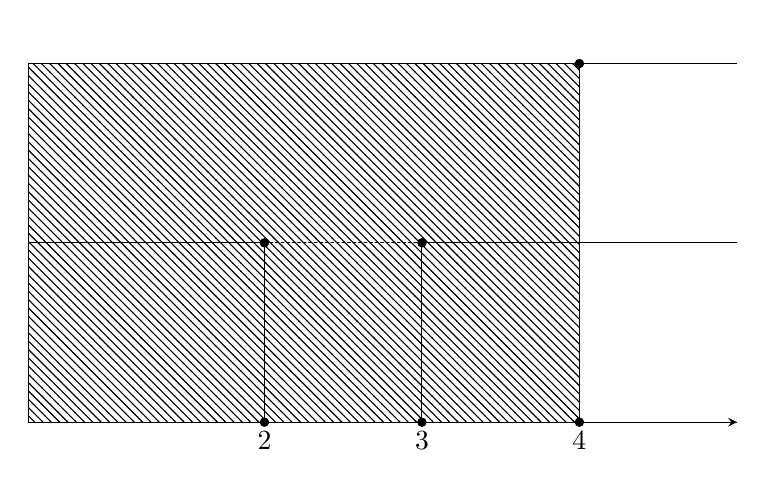
\begin{tikzpicture}[line cap=round,line join=round,>=triangle 45,x=1.0cm,y=1.0cm]
\begin{axis}[
x=1.0cm,%y=1.0cm,
axis x line=middle,
axis y line=none,
ticks=none,
%ymajorgrids=true,
%xmajorgrids=true,
xmin=0.0,
xmax=9.0,
ymin=-0.3,
ymax=2.2,
%xtick={0.0,1.0,...,10.0},
%ytick={-1.0,0.0,...,3.0},
]
\clip(0.,-0.3) rectangle (9.,2.2);
\draw  (0.,0.)-- (9.,0.);
\draw  (0.,1.)-- (3.,1.);
\draw  (5.,1.)-- (9.,1.);
\draw [dash pattern=on 1pt off 1pt] (3.,1.)-- (5.,1.);
\draw [dash pattern=on 1pt off 1pt] (0.,2.)-- (7.,2.);
\draw  (7.,2.)-- (9.,2.);
\draw  (7.,2.)-- (7.,0.);
\draw  (5.,1.)-- (5.,0.);
\draw  (3.,1.)-- (3.,0.);
\begin{scriptsize}
\draw[pattern=north west lines] (0,0) rectangle (7,2);
\draw [fill=black] (3.,0.) circle (1.5pt);
\draw[color=black] (3.0,-0.1) node {$2$};
\draw [fill=black] (3.,1.) circle (1.5pt);

\draw [fill=black] (5.,1.) circle (1.5pt);

\draw [fill=black] (5.,0.) circle (1.5pt);
\draw[color=black] (5.0,-0.1) node {$3$};
\draw [fill=black] (7.,0.) circle (1.5pt);
\draw[color=black] (7.0,-0.1) node {$4$};
\draw [fill=black] (7.,2.) circle (1.5pt);


\end{scriptsize}
\end{axis}
\end{tikzpicture}
\end{document}